% This code is a tweaked version of the script generated by GeoGebra (https://www.geogebra.org/)
% arara: latexmk: {options: [-pv]}
% arara: indent: {overwrite: yes, silent: yes, cruft: build}
\documentclass[tikz, border = 1pt]{standalone}

\usepackage{pgf, pgfplots}
\pgfplotsset{compat = 1.15}
\usepackage{mathrsfs}
\usetikzlibrary{arrows}

\definecolor{shadeofgreen}{HTML}{4daf4a}
\definecolor{shadeofred}{HTML}{e41a1c}
\definecolor{shadeofblue}{HTML}{377eb8}

\begin{document}
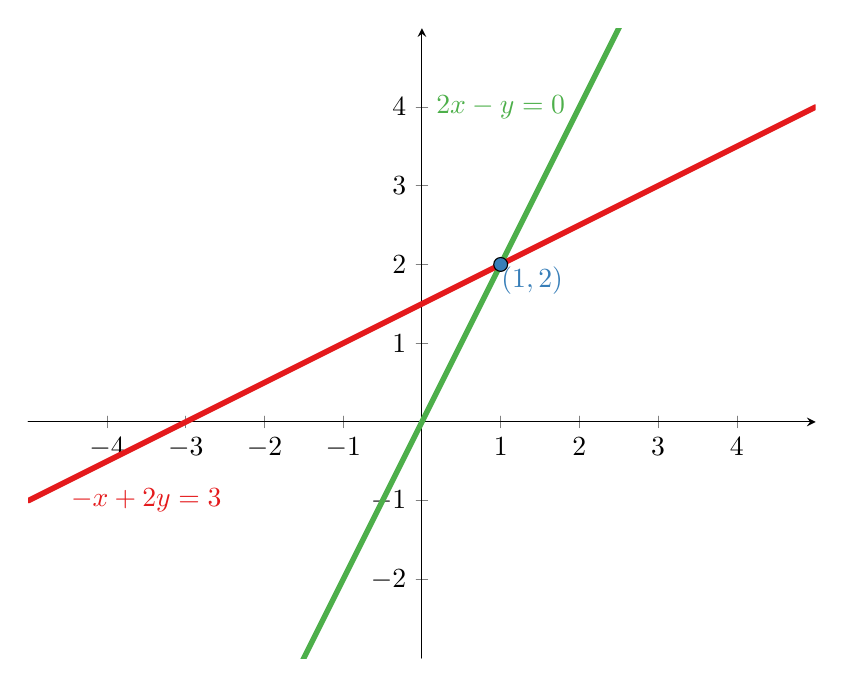
\begin{tikzpicture}[line cap = round, line join = round, >=triangle 45, x = 1cm, y = 1cm]
	\begin{axis}[
			x = 1cm, y = 1cm,
			axis lines = middle,
			xmin = -5,
			xmax = 5,
			ymin = -3,
			ymax = 5,
			xtick = {-4,..., 4},
			ytick = {-2,..., 4}
		]
		\clip(-5, -3) rectangle (5, 5);
		\draw [line width = 2pt, color = shadeofgreen, domain = -5:5] plot(\x,{(-0-2*\x)/-1});
		\draw [line width = 2pt, color = shadeofred, domain = -5:5] plot(\x,{(--3--1*\x)/2});
		\begin{scriptsize}
			\draw[color = shadeofgreen] (1, 4) node {\(2x - y = 0\)};
			\draw[color = shadeofred] (-3.5, -1) node {\(-x + 2y = 3\)};
			\draw[fill = shadeofblue] (1, 2) circle (2.5pt);
			\draw[color = shadeofblue] (1.4, 1.8) node {\((1, 2)\)};
		\end{scriptsize}
	\end{axis}
\end{tikzpicture}
\end{document}